\documentclass[10pt,a4paper]{article}
\usepackage{times}                       % 使用 Times New Roman 字体
\usepackage{CJK,CJKnumb,CJKulem}         % 中文支持宏包
\usepackage{color}                       % 支持彩色

\usepackage{comment}
\usepackage{amsmath}
\usepackage{amsfonts}
\usepackage{amssymb}
\usepackage{amsthm}
\usepackage{amscd}
\usepackage{mathtools}
\usepackage{graphicx}
\usepackage{indentfirst}
\usepackage{titlesec}
\usepackage[top=25.4mm, bottom=25.4mm, left=31.7mm, right=32.2mm]{geometry}

%\usepackage{natbib}
\usepackage{chapterbib}
\usepackage{bm}
\usepackage{url}
\usepackage{subfig}
%\usepackage[]{hyperref}

%页面设置
\begin{CJK*}{UTF8}{wqyzh}
%\theoremstyle{definition}
%\newtheoremstyle{mythm}{1.5ex plus 1ex minus .2ex}{1.5ex plus 1ex minus .2ex}
%   {\kai}{\parindent}{\wqyzh\bfseries}{}{1em}{}
\newtheoremstyle{mythm}{1ex}{1ex}%定理环境的上下间距.
{\CJKfamily{wqyzh}}{\parindent}{\CJKfamily{wqyzh} \bf}{}{1em}{}%定理内容为宋体, 缩进, 定理名称为黑粗体
\theoremstyle{mythm}%设置定理环境
\newtheorem{thm}{定理~}[section]
\newtheorem{lem}[thm]{引理~}
\newtheorem{pro}[thm]{性质~}
\newtheorem{fact}[thm]{Fact}
\newtheorem{prop}[thm]{命题~}
\newtheorem{ques}[thm]{问题~}
\newtheorem{cor}[thm]{推论~}
\newtheorem{de}[thm]{定义~}
\newtheorem{rem}[thm]{注记~}
\numberwithin{equation}{section}
\end{CJK*}
\renewcommand\refname{\CJKfamily{wqyzh}参考文献}
\renewcommand{\figurename}{图}
%\renewcommand{\abstractname}{摘要}
%%%%%%%%%%%%%%%%下面几行用于改变证明环境的定义
\makeatletter
\renewenvironment{proof}[1][\proofname]{\par
\pushQED{\qed}%
\normalfont \topsep6\p@\@plus6\p@ \labelsep1em\relax
\trivlist
\item[\hskip\labelsep\indent
\bfseries #1]\ignorespaces
}{%
\popQED\endtrivlist\@endpefalse
}
\makeatother
%%%%%%%%%%%%%%(http://latex.yo2.cn)
\renewcommand{\proofname}{\CJKfamily{wqyzh}证明}

\renewcommand{\thefootnote}{\fnsymbol{footnote}}
%\titleformat{\section}{\CJKfamily{wqyzh} }{\arabic{section}{1em}{}
\titleformat{\section}{\large \bf \CJKfamily{wqyzh} }{{\bf \thesection\space}}{0pt}{}

\DeclarePairedDelimiter\abs{\lvert}{\rvert}%
\DeclarePairedDelimiter\norm{\lVert}{\rVert}%

%\clearpage % 换页,\newpage也可以,推荐\clearpage

\begin{document}
%\setlength{\baselineskip}{1ex}%设置行距
\setlength{\abovedisplayskip}{1ex} %设置公式上边间距
\setlength{\belowdisplayskip}{1ex} %设置公式下边间距
\begin{CJK*}{UTF8}{wqyzh}

\author{陈鹏宇 (3100000140)}                                 % 作者
\title{计算机应用数学的作业报告}              % 题目
\maketitle                                           % 生成标题

\section*{说明}

\subparagraph{关于图形绘制的库}

几次作业均使用Python完成,在Python~3.4.1中进行了测试。我没有使用gnuplot,而是
使用matplotlib进行作图,因我对后者更加习惯,并且后者没有什么明显不如前者的地方
。

\subparagraph{关于报告中的字体}

simsun等一些模板中指定的字体并不是自由(free)或免费(free)的,只不过通常情况下随
着MS~Windows等软件产品的分发,其协议中已经许可了对其中附带的字体的使用。但我的
笔记本在收到后已经删除了OEM的MS~Windows操作系统并安装了GNU/Linux,尽管仍然可以
从互联网获得字体文件,但对其的使用是侵权行为。因此我使用了文泉驿正黑体这款自由
字体来完成本文。

事实上我也可以通过将我现有的MS~Windows操作系统安装到我的电脑上并从中提取字体文
件的方法来合法地获得模板中要求的字体,但这种方法代价稍大,需花费额外的时间,并
需格式化我的部分硬盘空间。权衡之后我暂时使用了现在这种自由字体的解决方案。

\section{曲线拟合}

\subsection{方法概述}

\subsubsection{最小二乘方法求解曲线拟合}

给定了一组容量为$n$的采样点$x_i, y_i$,假定采用次数为$d$的多项式函数对其进行拟
合。首先构造矩阵$X_{n\times d}$,其中$X_{i j} = x_i^{j-i}$,则这一拟合问题可被
表示为通过对误差函数
\begin{equation}
    E(a) = \norm{Xa - y}
\end{equation}
的最小化,对系数向量$a$的求解。则令其导数为零,由
\begin{equation}
    E'(a) = 0
\end{equation}
可以解得
\begin{equation}
    a = (X^T X)^{-1}Xy
\end{equation}
即求解得到所需的$a$。

\subsubsection{引入了正则项约束的误差函数}

在上面的方法中,$n$与$d$相差不多时往往出现过拟合的问题。因此我们可以改进误差函
数,将一个用于约束的正则项引入进去,得到
\begin{equation}
    E_1(a) = \norm{Xa - y} + \lambda \norm{a}
\end{equation}
此时可以解得
\begin{equation}
    a = (X^T X + \lambda I)^{-1}Xy
\end{equation}
此时得到的效果中过拟合现象就可以得到减轻。

\subsection{实验结果}

实验中我们采取$f = sin(x)$在区间$0, 2\pi$上作为目标函数,通过在数据点上施加随
机误差来得到有误差的采样点,随后使用我们的方法进行拟合。图\ref{fig:curve-fit}
给出了拟合的结果

\begin{figure}[h]
    \centering
    \def\_width{0.33\textwidth}
    \subfloat[$d=3$,$n=10$]{
        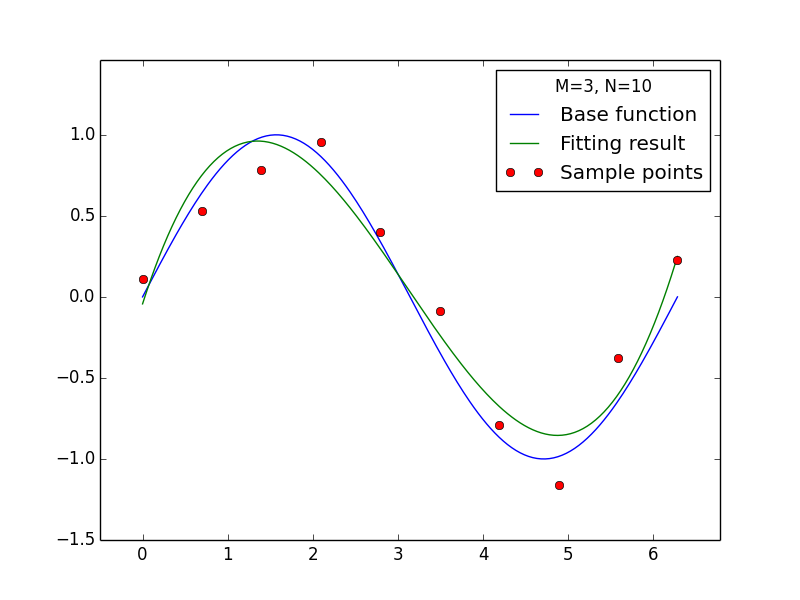
\includegraphics[width=\_width]{figs/curve-fit-0.png}
    }
    \subfloat[$d=9$,$n=10$]{
        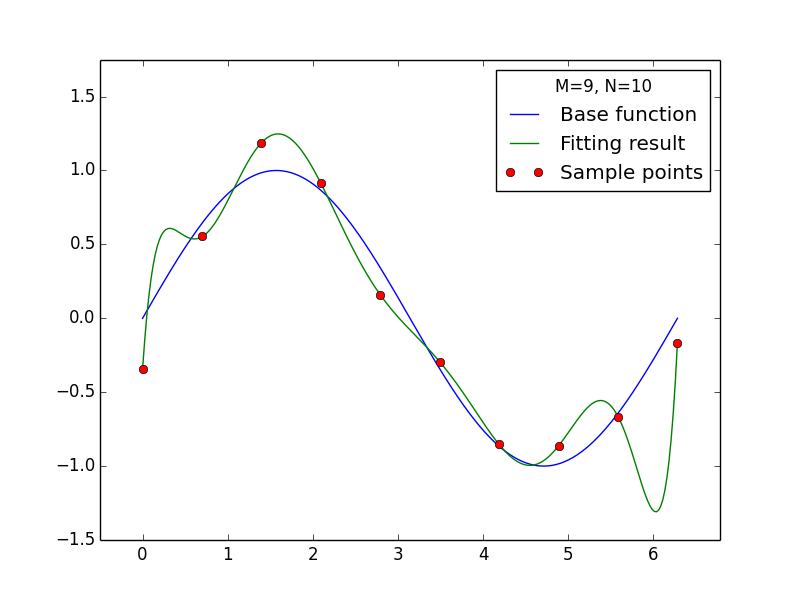
\includegraphics[width=\_width]{figs/curve-fit-1.png}
    }
    \subfloat[$d=9$,$n=15$]{
        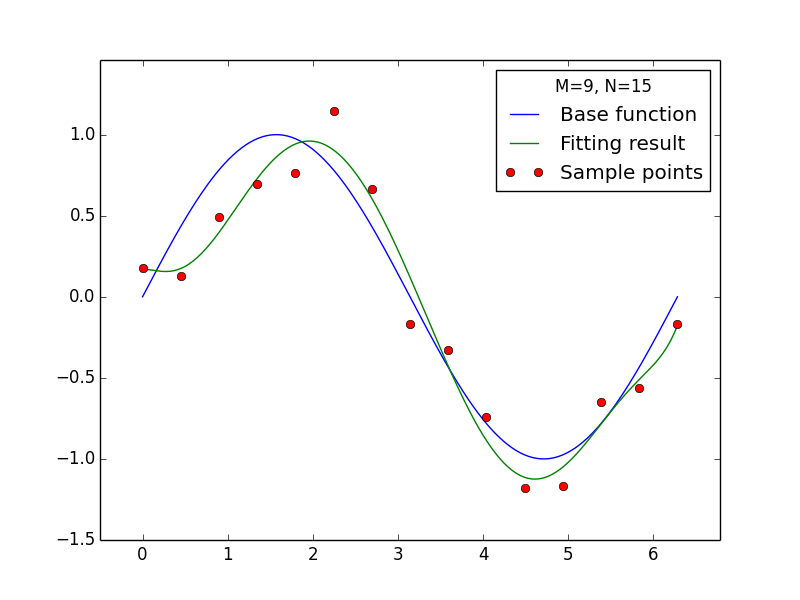
\includegraphics[width=\_width]{figs/curve-fit-2.png}
    }
    \\
    \subfloat[$d=9$,$n=100$]{
        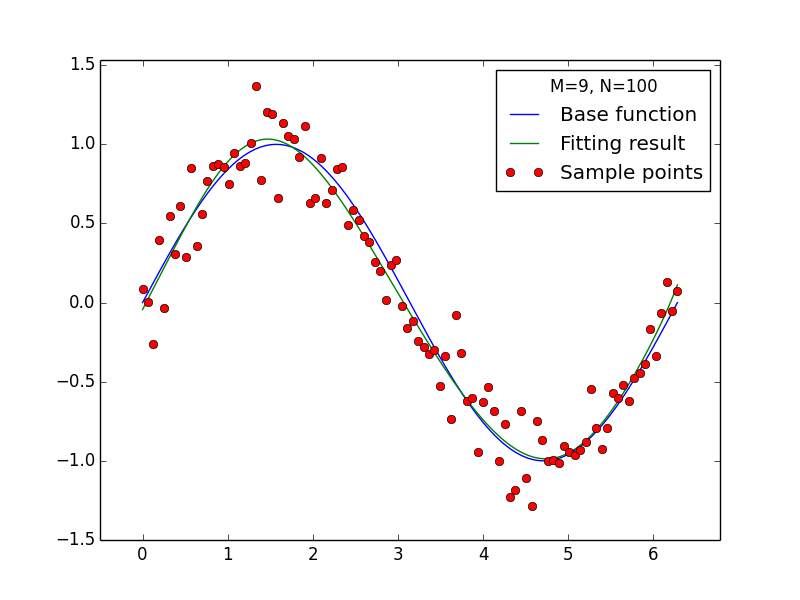
\includegraphics[width=\_width]{figs/curve-fit-3.png}
    }
    \subfloat[$d=9$,$n=100$,$\log \lambda = -4$]{
        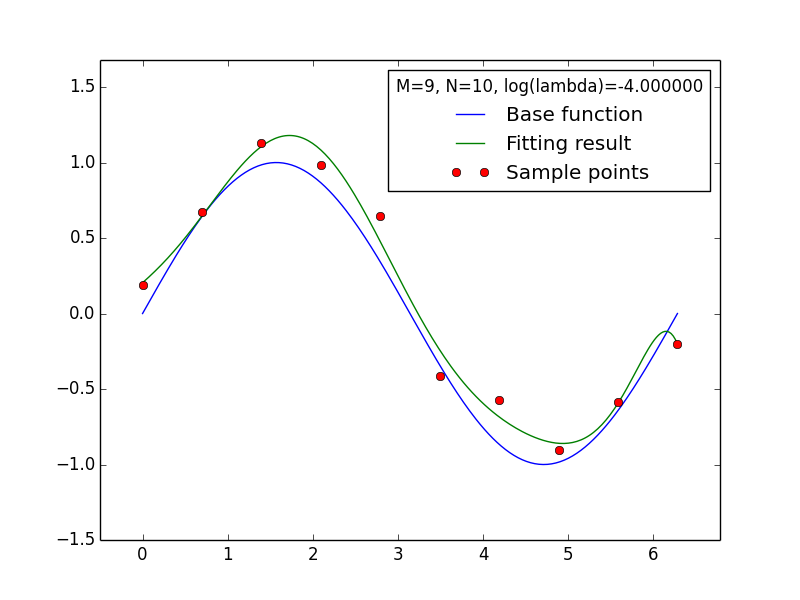
\includegraphics[width=\_width]{figs/curve-fit-4.png}
    }
    \caption{
        一些不同参数曲线拟合的对比,从中可以明显看出过拟合的效果
    }{}
    \label{fig:curve-fit}
\end{figure}

\subsection{小结与讨论}
由图\ref{fig:curve-fit}可以看出,对于同样的多项式次数$d$,增加样本容量$n$将提
高拟合精度。而当$d$与$n$相差不多时,过拟合的问题将被引入,从而导致拟合程度降低
。而正则项的加入可以在一定程度上解决这一问题。

注意到在实验中我们使用了高达$d=9$次的多项式来进行拟合,这就在浮点数运算上引入
了不小的误差。将函数定义域从$[0,2\pi)$调整到$[0,1)$可以在一定程度上减轻这个问
题。

\section{主成分分析}

\subsection{方法概述}

我们从UCI提供的数据集
\footnote{\url{http://archive.ics.uci.edu/ml/datasets/Optical+Recognition+of+Handwritten+Digits}}
下载采集到的手写数据集,并选择其中未经处理的数据中全部共572份数字3的数据作为我们的数
据集。数据集中每一份采样是$32\times 32$的二值矩阵,我们将其视为一个1024维的向
量,因此全部数据构成一个$572\times 1024$的矩阵,将其中心平移到原点得到矩阵$A$。

这里主成分分析的目标是将我们的数据$A$投影到新的维度上,使在新的一组基下,基的
方向与数据的矩阵$A$的特征值降序的排列一致。即只需对其进行SVD分解:
\begin{equation}
    Y = U D V^T
\end{equation}
其中$U$与$V$为正交矩阵,$D$为对角阵且其对角元素为降序排列的$Y$的奇异值。在SVD
分解的前提下,选取前若干个奇异值对应的特征方向,将数据投影到以这些方向为基的空
间中,即可有效地完成降维的目的。在实验中我们选取前两个特征方向,将数据投影到二
维空间中。


\subsection{实验结果}

图\ref{fig:pca}给出了将输入的572张图像投影到二维的情况,图\ref{fig:pca-1}给出
了原始数据投影到住分量所在的空间中的分布,图\ref{fig:pca-2}给出了用对应的两个
主分量表示的数据,从中似乎可以看出一些倾斜与笔画的变化,但并不明显。关于这一现
象我们将在第\ref{sec:2nd-conclusion}中进行分析与讨论。

\begin{figure}[h]
    \centering
    \def\_width{0.32\textwidth}
    \subfloat[将输入数据投影到二维中的情况]{
        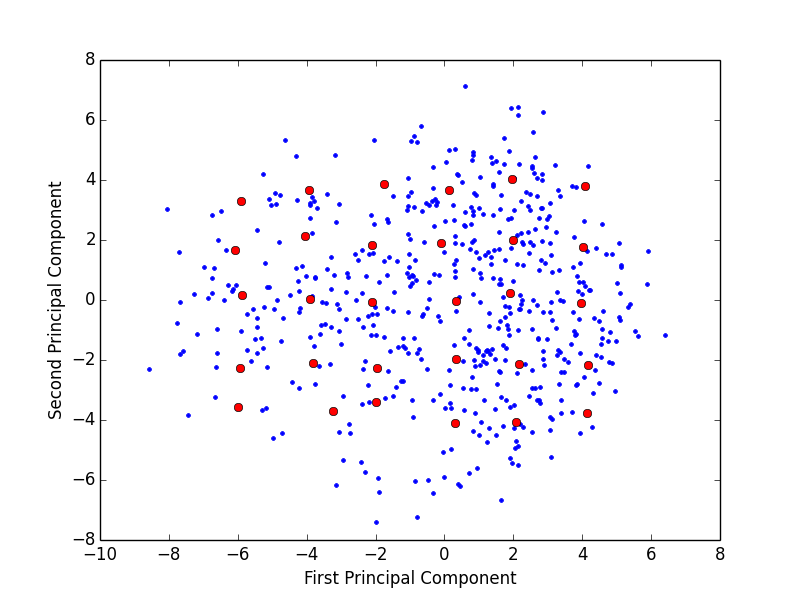
\includegraphics[width=\_width]{figs/pca-0.png}
        \label{fig:pca-0}
    }
    \subfloat[一些采样的点的原始图像]{
        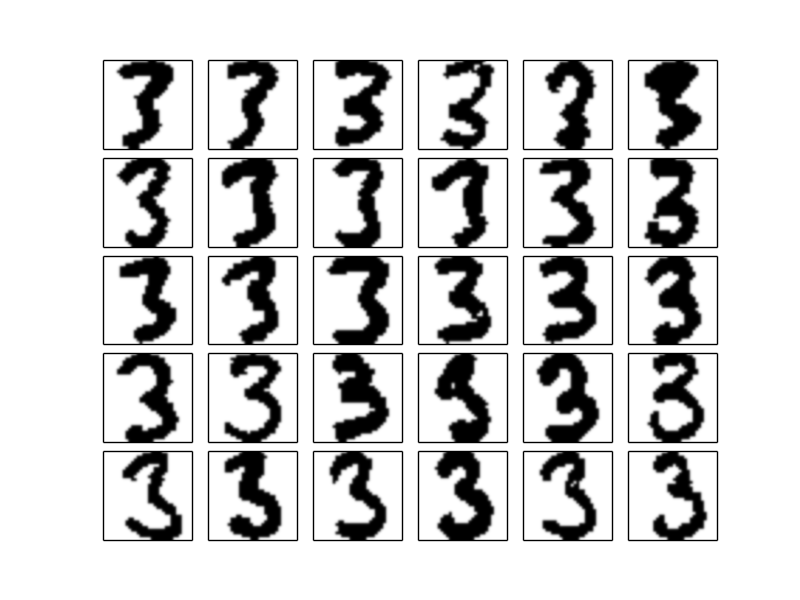
\includegraphics[width=\_width]{figs/pca-1.png}
        \label{fig:pca-1}
    }
    \subfloat[一些采样的点投影在两个特征向量所张成的空间中的图像]{
        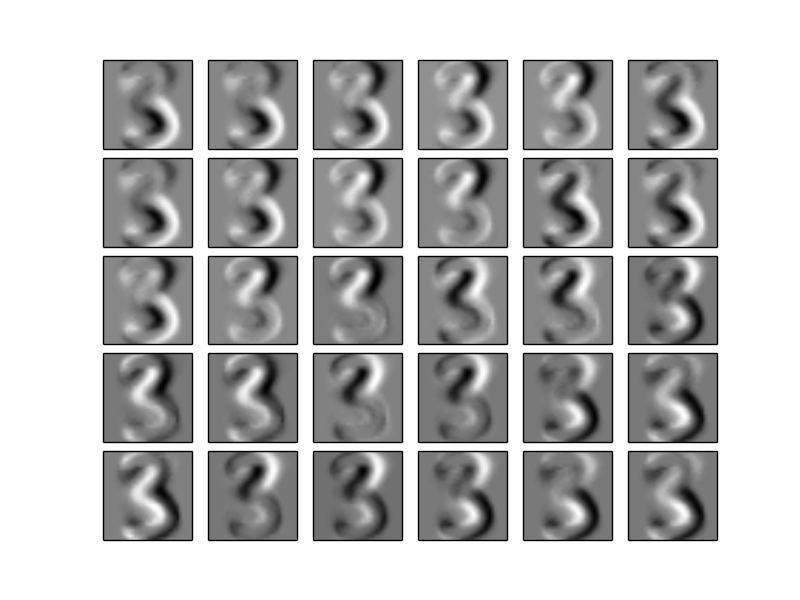
\includegraphics[width=\_width]{figs/pca-2.png}
        \label{fig:pca-2}
    }
    \caption{
    }{}
    \label{fig:pca}
\end{figure}


\subsection{小结与讨论}

\label{sec:2nd-conclusion}

我们对于输入数据进行了矢量化的表示并进行了奇异值分解,在得到的结果上取前两个特
征值并将原数据投影到相应的特征向量组成的空间中,从而进行在主要分量上的降维处理
。但图\ref{fig:pca}中给出的结果似乎并不明显。

PCA对数据的特征的缩放十分敏感,因此当从原始数据转换得到欧式空间中被用来处理的
向量时,往往需要寻求合适的表示方法,并在例如长度、重量、时间等已知的特征上对方
差进行归一化处理。在实验中我们直接将$32 \times 32$的图片视为$1024$维的像素向量
,这可能是引入较大误差的地方。

但可惜的是,尽管我们又做了一些实验,使用不同的采样与表达方式来对原始数据进行处
理,但从结果上看PCA并没有给出太令人满意的例子。也许是我们使用的数据集本身噪声
就很大,也有可能是我们选用的采样方法并不合适。



\section{混合高斯模型的生成与基于期望最大化方法的求解}

\subsection{方法概述}

在一维情况的标准高斯分布前提下,独立采样$n$次得到向量$X$,则向量$LX + \mu$为
$n$元高斯分布$N(X;\mu, \Sigma)$的样本,其中$L$是满足$LL^T=\Sigma$的矩阵。

而对于混合高斯模型
\begin{equation}
    p(X) = \sum_i p_i N(X;\mu_i, \Sigma_i)
\end{equation}
的采样,我们只需要依概率$p_i$对相应的高斯分布进行采样并组合即可。

而对于给定数据的求解,我们使用基于期望最大化的方法进行计算,依照课堂上讲稿中给
出的步骤进行计算
\footnote{\url{http://www.cad.zju.edu.cn/home/zhx/csmath/lib/exe/fetch.php?media=2014:csmath-03-distance_and_similarity.pdf}
,第54至57页}


\subsection{实验结果}

在某次实验中,我们采用如下的参数来生成1000个采样点:

\begin{verbatim}
Ground truth:
p:
0.5
0.3
0.2
mu:
[4 1]
[-2  3]
[0 0]
sigma:
[[ 1.2 -0.4]
 [-0.4  1.2]]
[[ 1.   0.2]
 [ 0.2  1. ]]
[[ 1.   0.7]
 [ 0.7  1. ]]
\end{verbatim}

\begin{figure}[h]
    \centering
    \def\_width{0.75\textwidth}
    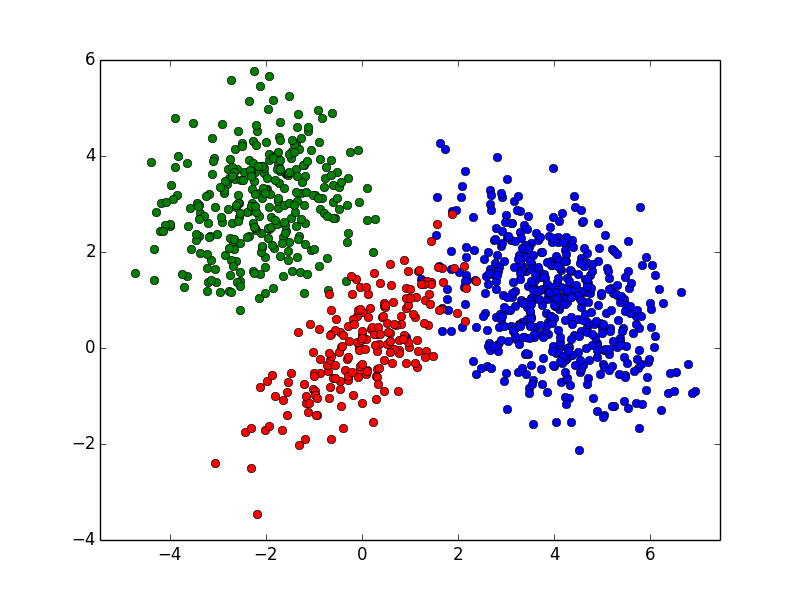
\includegraphics[width=\_width]{figs/gauss-0.png}
    \caption{
        由给定的参数采样得到的点的示例
    }{}
    \label{fig:gauss}
\end{figure}

在55次迭代后我们得到精度满足要求的解如下:
\begin{verbatim}
Estimation:
p:
0.492583328964
0.299899091702
0.207517579333
mu:
[ 4.04065041  0.92409708]
[-2.09735184  3.0385326 ]
[ 0.15332528  0.1345286 ]
sigma:
[[ 1.17923185 -0.43327161]
 [-0.43327161  1.23005181]]
[[ 0.97418514  0.16684165]
 [ 0.16684165  0.99325668]]
[[ 1.19464678  0.82832289]
 [ 0.82832289  1.05443236]]
\end{verbatim}

可以看出两者差别并不很大。

\subsection{小结与讨论}

我们用来生成样本的方法可以比较好地体现参数的特征,而我们的基于最大化概率的解法
可以解出比较接近原参数的解。

同时我们也对参数进行了多次调整,其结果与预期一致。当样本点数目增加时算法的结果
精度也会有相应地提升,但程序运行也会更加耗时。当调整参数使高斯分布之间重合部分
更大时,算法收敛速度明显变慢,同时解的精度下降。

算法的设计与实现事实上可以处理任意维度下任意个高斯分布的混合模型,这里取了二维
情况下三个高斯分布的混合作为例子来展示。


\section{非线性优化的LM方法求解}

\subsection{方法概述}

对于给定的函数$f(p)$,目标值$x$与初始点$p_0$,求解一个$p$使$\norm{f(p) - x}$最
小。其思路为在当前状态的一个邻域中取函数到二次的泰勒展开作为近似并进行求解。

我们对课程讲稿上描述的LM方法
\footnote{\url{http://www.cad.zju.edu.cn/home/zhx/csmath/lib/exe/fetch.php?media=2014:csmath-07-nonlinear.pdf}
第45至47页}进行了实现。

\subsection{实验结果}

我们使用LM算法进行了引入正规项的多项式拟合的计算,使用与实验一中相似的数据。图
\ref{fig:lm}给出了拟合的结果:

\begin{figure}[h]
    \centering
    \def\_width{0.75\textwidth}
    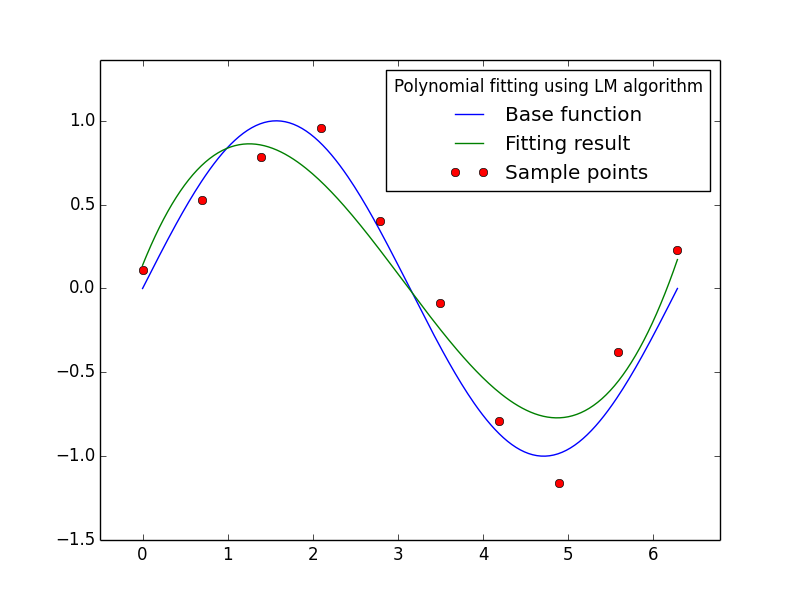
\includegraphics[width=\_width]{figs/lm-0.png}
    \caption{
        使用LM算法进行多项式拟合的示例
    }{}
    \label{fig:lm}
\end{figure}

\subsection{小结与讨论}

从原理上看,LM算法引入了$\mu$来使$G + \mu I$正定从而保证解严格最小,同时
$\mu$在迭代中的变化也使得算法在初期比较接近最速下降法,而在末期比较接近朴素的
牛顿方法。

但我们的实验中并没有对算法的收敛速度作进一步的研究。

%\bibliographystyle{alpha}
%\bibliography{paper}

\end{CJK*}
\end{document}
